\begin{frame}{Lists and emphasis}
  \begin{itemize}
    \setlength{\itemsep}{3mm}
    \item Plain text with \textbf{bold}, \emph{emphasis}, \alert{alerts} and \texttt{monospace}.
    \item Nested lists:
    \begin{itemize}
      \item second level is \texttt{\textbackslash small}
      \item and uses the same bullet
    \end{itemize}
    \item Enumerations:
    \begin{enumerate}
      \item first
      \item second
    \end{enumerate}
  \end{itemize}
\end{frame}

\begin{frame}{Overlays}
  \begin{itemize}
    \item Revealed step by step \pause
    \item with \texttt{\textbackslash pause} \pause
    \item and the preview shows step dots in the corner
  \end{itemize}
  \begin{center}
    \only<1>{Step one shows this text.}
    \only<2>{Step two replaces it.}
    \only<3>{Step three replaces it again.}
  \end{center}
\end{frame}

\begin{frame}{Math}
  \begin{itemize}
    \item Inline $E(X) = \sum_i p(x_i)\, x_i$ and a user macro $\norm{x}_2$.
    \item Display math:
    $$\hat{\beta} = \left(X^\top X\right)^{-1} X^\top y$$
    \item Aligned equations:
    \begin{align*}
      f(x) &= \frac{1}{\sigma\sqrt{2\pi}} e^{-\frac{(x-\mu)^2}{2\sigma^2}} \\
      \sigma(x) &= \frac{1}{1+e^{-x}}
    \end{align*}
  \end{itemize}
\end{frame}

\begin{frame}{Columns and images}
  \begin{columns}
    \begin{column}{0.45\textwidth}
      \begin{itemize}
        \item Left: a PNG image
        \item Right: a PDF figure, rendered with pdf.js
        \item Sizes follow \texttt{width=} / \texttt{height=}\footnote{Footnotes go to the bottom of the frame.}
      \end{itemize}
    \end{column}
    \begin{column}{0.5\textwidth}
      \centering
      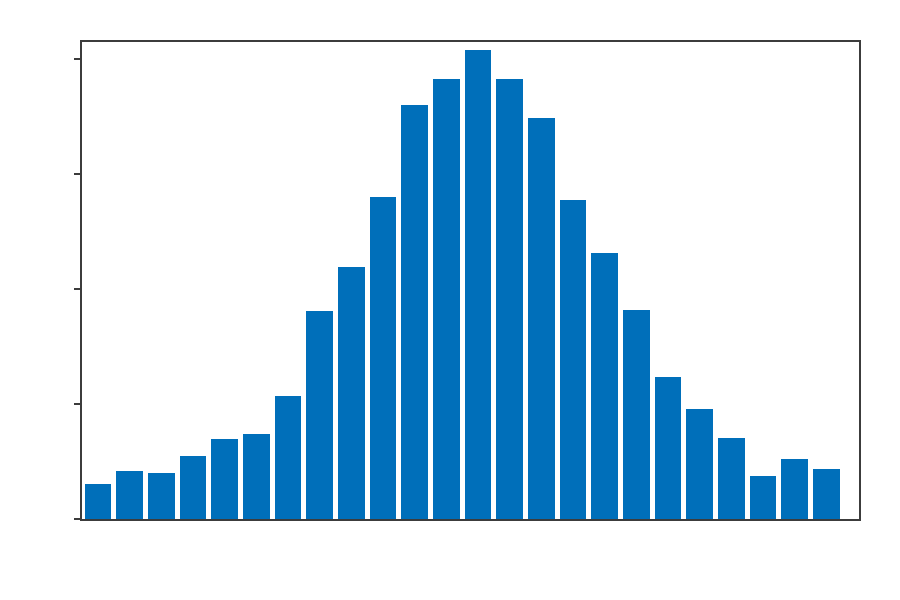
\includegraphics[width=0.8\textwidth]{../figures/histogram.png}\\[2mm]
      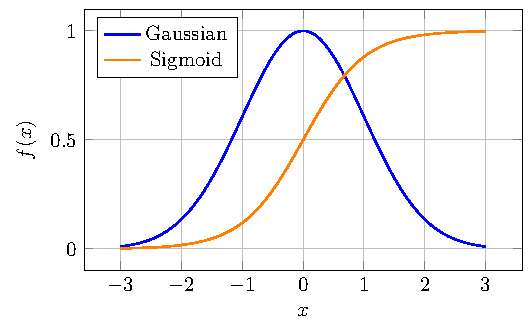
\includegraphics[width=0.9\textwidth]{../figures/curve.pdf}
    \end{column}
  \end{columns}
\end{frame}

\begin{frame}{Blocks}
  \begin{block}{Block}
    A regular block with \texttt{block=fill}.
  \end{block}
  \begin{alertblock}{Alert block}
    Titles use the alert colour.
  \end{alertblock}
  \begin{exampleblock}{Example block}
    Titles use the \texttt{example text} colour.
  \end{exampleblock}
\end{frame}
